\documentclass[11pt,letterpaper]{article}
\setlength{\parindent}{0em}                  %DISTANCIA SANGRÍA
\setlength{\parskip}{0.5em}                  %DISTANCIA ENTRE PÁRRAFOS
\textwidth 6.5in
\textheight 9.in
\oddsidemargin 0in
\headheight 0in

\usepackage{fancybox}
\usepackage[utf8]{inputenc}
\usepackage{epsfig,graphicx}
\usepackage{multicol,pst-plot}
\usepackage{pstricks}
\usepackage{amsmath}
\usepackage{amsfonts}
\usepackage{amssymb}
\usepackage{eucal}
\usepackage[left=2cm,right=2cm,top=2cm,bottom=2cm]{geometry}
\usepackage{txfonts}
% \usepackage[spanish]{babel}
\usepackage[colorlinks]{hyperref}
\usepackage{cancel}
\usepackage{caption}
\usepackage{float}
\usepackage{upgreek}
\usepackage{gensymb}
\usepackage{subfigure}
\usepackage{siunitx}
\usepackage{color}
\usepackage{tikz}
\usepackage{listings}
%\usepackage{minted}
\usepackage{mdframed}
\usepackage{natbib}
\usepackage{pifont}
\bibliographystyle{mnras}
\setcitestyle{aysep{","}}
\usepackage{multicol}
\renewcommand{\bibpreamble}{\begin{multicols}{2}}
\renewcommand{\bibpostamble}{\end{multicols}}
\setlength{\bibsep}{3pt}

%DEFINICIÓN DE COLORES EXTRAS

\definecolor{codegreen}{rgb}{0,0.6,0}
\definecolor{codegray}{rgb}{0.5,0.5,0.5}
\definecolor{backcolour}{rgb}{0.95,0.95,0.95}
\hypersetup{colorlinks=true,linkcolor=codegreen,citecolor=blue,filecolor=blue,urlcolor=magenta,}

%CONFIGURACIÓN DE LSTLISTINGS PARA CÓDIGOS

\lstset{ %
language=matlab,                % choose the language of the code
basicstyle=\footnotesize,       % the size of the fonts that are used for the code
numbers=left,                   % where to put the line-numbers
numberstyle=\footnotesize,      % the size of the fonts that are used for the line-numbers
stepnumber=1,                   % the step between two line-numbers. If it is 1 each line will be numbered
numbersep=5pt,                  % how far the line-numbers are from the code
backgroundcolor=\color{white},  % choose the background color. You must add \usepackage{color}
showspaces=false,               % show spaces adding particular underscores
showstringspaces=false,         % underline spaces within strings
showtabs=false,                 % show tabs within strings adding particular underscores
frame=single,                   % adds a frame around the code
tabsize=2,                      % sets default tabsize to 2 spaces
captionpos=b,                   % sets the caption-position to bottom
breaklines=true,                % sets automatic line breaking
breakatwhitespace=false,        % sets if automatic breaks should only happen at whitespace
escapeinside={\%*}{*)}          % if you want to add a comment within your code
}
\lstdefinestyle{mystyle}{
	backgroundcolor=\color{backcolour},   
	commentstyle=\color{red},
	keywordstyle=\bfseries\color{magenta},
	numberstyle=\tiny\color{codegray},
	stringstyle=\color{codegreen},
	basicstyle=\footnotesize\ttfamily,
	identifierstyle=\color{blue},
	breakatwhitespace=false,         
	breaklines=true,                 
	captionpos=b,                    
	keepspaces=true,                 
	numbers=left,                    
	numbersep=5pt,                  
	showspaces=false,                
	showstringspaces=false,
	showtabs=false,                  
	tabsize=2
}

\lstset{style=mystyle}

%CONFIGURACIÓN DE MINTED PARA CÓDIGOS

%\usemintedstyle{vs}

%DEFINICIÓN DE COMANDOS EXTRAS

\pagestyle{empty}
\DeclareMathOperator{\tr}{Tr}                      %ICONO TRAZA MECANICA CUANTICA
\DeclareMathOperator{\rsol}{R_\odot}               %ICONO RADIO SOLAR
\DeclareMathOperator{\lsol}{L_\odot}               %ICONO LUMINOSIDAD SOLAR
\DeclareMathOperator{\msol}{M_\odot}               %ICONO MASA SOLAR
\DeclareMathOperator{\probabi}{Prob}               %ICONO PROBABILIDAD
\newcommand{\units}[1]{\left[ #1 \right]}          %CORCHETES PARA UNIDADES
\newcommand{\prob}[1]{\probabi\left( #1 \right)}   %OPERADOR PROBABILIDAD
\newcommand{\abs}[1]{\left|#1\right|}              %OPERADOR VALOR ABSOLUTO
\newcommand{\bra}[1]{\langle #1 |}                 %OPERADOR BRA
\newcommand{\ket}[1]{| #1 \rangle}                 %OPERADOR KET
\newcommand{\braket}[2]{\langle #1 | #2 \rangle}   %OPERADOR BRA-KET
\newcommand{\ketbra}[2]{|#1\rangle\langle#2|}      %OPERADOR KET-BRA
\newcommand{\mean}[1]{\langle #1 \rangle}          %PROMEDIO MECANICA CUANTICA
\newcommand{\eval}[3]{\left.#1\right|_{#2}^{#3}}   %COMANDO PARA EVALUAR INTEGRALES

%DEFINICIÓN DE REVISTAS CIENTÍFICAS

\newcommand\aap{A\&A}                % Astronomy and Astrophysics
\let\astap=\aap                          % alternative shortcut
\newcommand\aapr{A\&ARv}             % Astronomy and Astrophysics Review (the)
\newcommand\aaps{A\&AS}              % Astronomy and Astrophysics Supplement Series
\newcommand\actaa{Acta Astron.}      % Acta Astronomica
\newcommand\afz{Afz}                 % Astrofizika
\newcommand\aj{AJ}                   % Astronomical Journal (the)
\newcommand\ao{Appl. Opt.}           % Applied Optics
\let\applopt=\ao                         % alternative shortcut
\newcommand\aplett{Astrophys.~Lett.} % Astrophysics Letters
\newcommand\apj{ApJ}                 % Astrophysical Journal
\newcommand\apjl{ApJ}                % Astrophysical Journal, Letters
\let\apjlett=\apjl                       % alternative shortcut
\newcommand\apjs{ApJS}               % Astrophysical Journal, Supplement
\let\apjsupp=\apjs                       % alternative shortcut
% The following journal does not appear to exist! Disabled.
%\newcommand\apspr{Astrophys.~Space~Phys.~Res.} % Astrophysics Space Physics Research
\newcommand\apss{Ap\&SS}             % Astrophysics and Space Science
\newcommand\araa{ARA\&A}             % Annual Review of Astronomy and Astrophysics
\newcommand\arep{Astron. Rep.}       % Astronomy Reports
\newcommand\aspc{ASP Conf. Ser.}     % ASP Conference Series
\newcommand\azh{Azh}                 % Astronomicheskii Zhurnal
\newcommand\baas{BAAS}               % Bulletin of the American Astronomical Society
\newcommand\bac{Bull. Astron. Inst. Czechoslovakia} % Bulletin of the Astronomical Institutes of Czechoslovakia 
\newcommand\bain{Bull. Astron. Inst. Netherlands} % Bulletin Astronomical Institute of the Netherlands
\newcommand\caa{Chinese Astron. Astrophys.} % Chinese Astronomy and Astrophysics
\newcommand\cjaa{Chinese J.~Astron. Astrophys.} % Chinese Journal of Astronomy and Astrophysics
\newcommand\fcp{Fundamentals Cosmic Phys.}  % Fundamentals of Cosmic Physics
\newcommand\gca{Geochimica Cosmochimica Acta}   % Geochimica Cosmochimica Acta
\newcommand\grl{Geophys. Res. Lett.} % Geophysics Research Letters
\newcommand\iaucirc{IAU~Circ.}       % IAU Cirulars
\newcommand\icarus{Icarus}           % Icarus
\newcommand\japa{J.~Astrophys. Astron.} % Journal of Astrophysics and Astronomy
\newcommand\jcap{J.~Cosmology Astropart. Phys.} % Journal of Cosmology and Astroparticle Physics
\newcommand\jcp{J.~Chem.~Phys.}      % Journal of Chemical Physics
\newcommand\jgr{J.~Geophys.~Res.}    % Journal of Geophysics Research
\newcommand\jqsrt{J.~Quant. Spectrosc. Radiative Transfer} % Journal of Quantitiative Spectroscopy and Radiative Transfer
\newcommand\jrasc{J.~R.~Astron. Soc. Canada} % Journal of the RAS of Canada
\newcommand\memras{Mem.~RAS}         % Memoirs of the RAS
\newcommand\memsai{Mem. Soc. Astron. Italiana} % Memoire della Societa Astronomica Italiana
\newcommand\mnassa{MNASSA}           % Monthly Notes of the Astronomical Society of Southern Africa
\newcommand\mnras{MNRAS}             % Monthly Notices of the Royal Astronomical Society
\newcommand\na{New~Astron.}          % New Astronomy
\newcommand\nar{New~Astron.~Rev.}    % New Astronomy Review
\newcommand\nat{Nature}              % Nature
\newcommand\nphysa{Nuclear Phys.~A}  % Nuclear Physics A
\newcommand\pra{Phys. Rev.~A}        % Physical Review A: General Physics
\newcommand\prb{Phys. Rev.~B}        % Physical Review B: Solid State
\newcommand\prc{Phys. Rev.~C}        % Physical Review C
\newcommand\prd{Phys. Rev.~D}        % Physical Review D
\newcommand\pre{Phys. Rev.~E}        % Physical Review E
\newcommand\prl{Phys. Rev.~Lett.}    % Physical Review Letters
\newcommand\pasa{Publ. Astron. Soc. Australia}  % Publications of the Astronomical Society of Australia
\newcommand\pasp{PASP}               % Publications of the Astronomical Society of the Pacific
\newcommand\pasj{PASJ}               % Publications of the Astronomical Society of Japan
\newcommand\physrep{Phys.~Rep.}      % Physics Reports
\newcommand\physscr{Phys.~Scr.}      % Physica Scripta
\newcommand\planss{Planet. Space~Sci.} % Planetary Space Science
\newcommand\procspie{Proc.~SPIE}     % Proceedings of the Society of Photo-Optical Instrumentation Engineers
\newcommand\rmxaa{Rev. Mex. Astron. Astrofis.} % Revista Mexicana de Astronomia y Astrofisica
\newcommand\qjras{QJRAS}             % Quarterly Journal of the RAS
\newcommand\sci{Science}             % Science
\newcommand\skytel{Sky \& Telesc.}   % Sky and Telescope
\newcommand\solphys{Sol.~Phys.}      % Solar Physics
\newcommand\sovast{Soviet~Ast.}      % Soviet Astronomy (aka Astronomy Reports)
\newcommand\ssr{Space Sci. Rev.}     % Space Science Reviews
\newcommand\zap{Z.~Astrophys.}       % Zeitschrift fuer Astrophysik

%COMIENZA EL DOCUMENTO

\begin{document}

%CONFIGURACIÓN DEL ENCABEZADO

\usetikzlibrary{positioning}
\tikzset{every picture/.style={line width=0.75pt}}    
\pagestyle{plain}
\begin{flushleft}
Digital Image Processing\\
School of Information Science and Technology\\
\underline{ShanghaiTech University}
\end{flushleft}

% \begin{flushright}\vspace{-5mm}
% \includegraphics[height=1.5cm]{shanghaitech.jpg}
% \end{flushright}
 
\begin{center}\vspace{-1cm}
\textbf{\large Assignment 3}\\  
Due time: 23:59,	May 5th,	2023\\
\end{center}
\rule{\linewidth}{0.1mm}

\section{Notes}
This homework has \textbf{80 points} in total. \par
Please submit your homework to blackboard with a zip file named as \textcolor[rgb]{1,0,0}{\textbf{DIP2023\_ID\_Name\_hw3.zip}}. The zip file should contain three things: \textcolor[rgb]{1,0,0}{\textbf{a folder named 'codes' storing your codes}},  \textcolor[rgb]{1,0,0}{\textbf{a folder named 'images' storing the original images}}, and \textcolor[rgb]{1,0,0}{\textbf{your report named as report\_ID\_Name\_hw3.pdf}}. The names of your codes should look like \textcolor[rgb]{1,0,0}{\textbf{'p1a.m'}} (for (a) part of Problem $1$), so that we can easily match your answer to the question. \textcolor[rgb]{1,0,0}{Make sure all paths in your codes are relative path and we can get the result directly after running the code}. Please answer in \textcolor[rgb]{1,0,0}{English}. \par

Please complete all the coding assignments using \textcolor[rgb]{1,0,0}{MATLAB}. All core codes are required to be implemented \textcolor[rgb]{1,0,0}{by yourself} (without using relevant built-in functions). Make sure your results in the report are the same with the results of your codes. Please explain with notes at least at the key steps of your code.

\section{Policy on plagiarism}
This is an individual homework. You can discuss the ideas and algorithms, but you can neither read, modify, and submit the codes of other students, nor allow other students to read, modify, and submit your codes. Do not directly copy ready-made or automatically generated codes, or your score will be seriously affected. We will check plagiarism using automated tools and any violations will result in a zero score for this assignment. 

\clearpage


\subsection*{Problem 1 (30 pts)}

\begin{itemize}
\item[(a)] Please implement the Basic global thresholding on "flower.tif". (start with T = 0.001) (10pts)

\item[(b)] Please implement the Otsus method on "caster\_stand.tif". (10 pts)

\item[(c)] Please implement the edge tracking using Canny Edge Detector on "fingerprint.tif". (10 pts)
\end{itemize}
\textbf{Solution:}
\begin{itemize}
	\item [(a)] The binarized image is shown in Figure~\ref{fig:p1a}.
	\item [(b)] The binary image processed by Otsus method is shown in Figure~\ref{fig:p1b}.
	\item [(c)] The edge tracking result using Canny Edge Detector is shown in Figure~\ref{fig:p1c}.
				The gaussian filter has size $30\times 30$ and $\sigma=5$. The low and high thresholding is 0.2 and 0.48.
\end{itemize}
\begin{figure}[htpb]
	\centering
	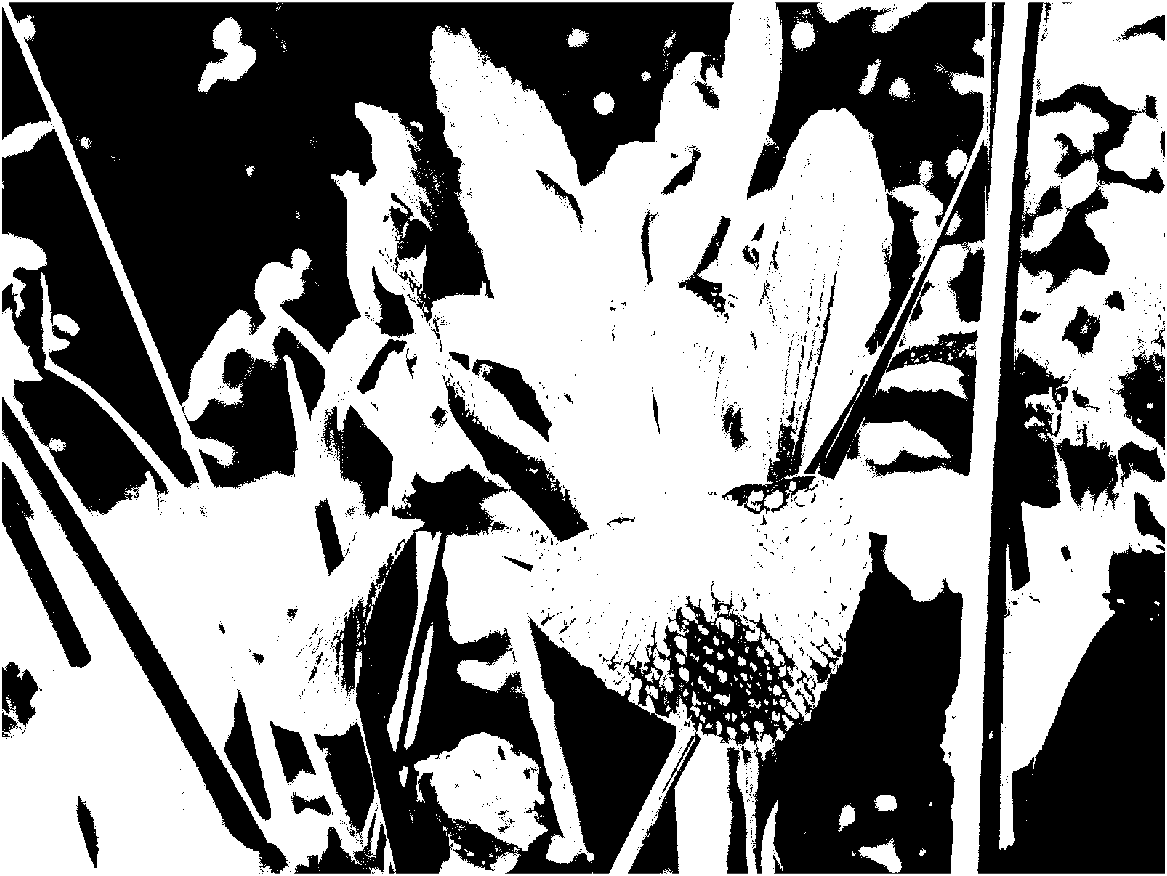
\includegraphics[height=0.4\textwidth]{../images/p1a/p1a.png}
	\caption{Basic global thresholding on "flower.tif}
	\label{fig:p1a}
	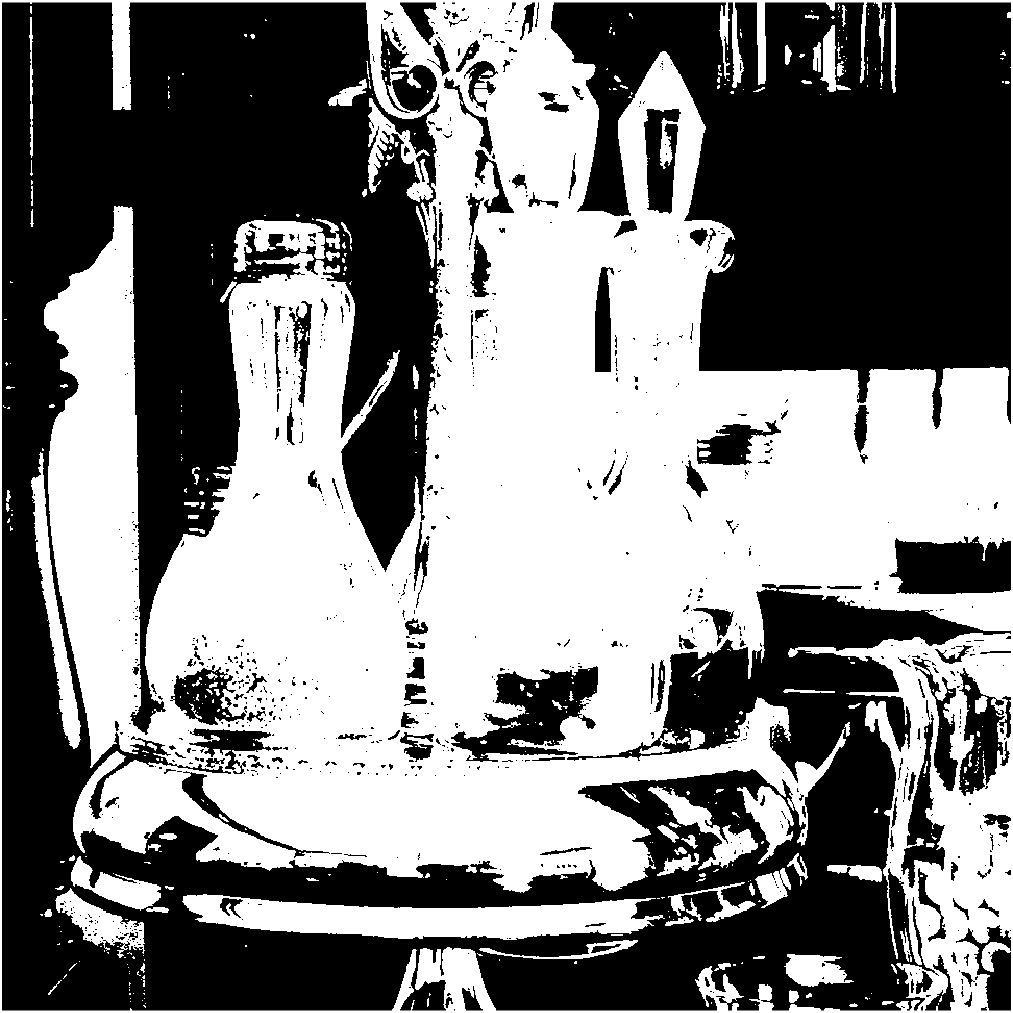
\includegraphics[height=0.4\textwidth]{../images/p1b/p1b.png}
	\caption{Otsus method on "caster\_stand.tif}
	\label{fig:p1b}
	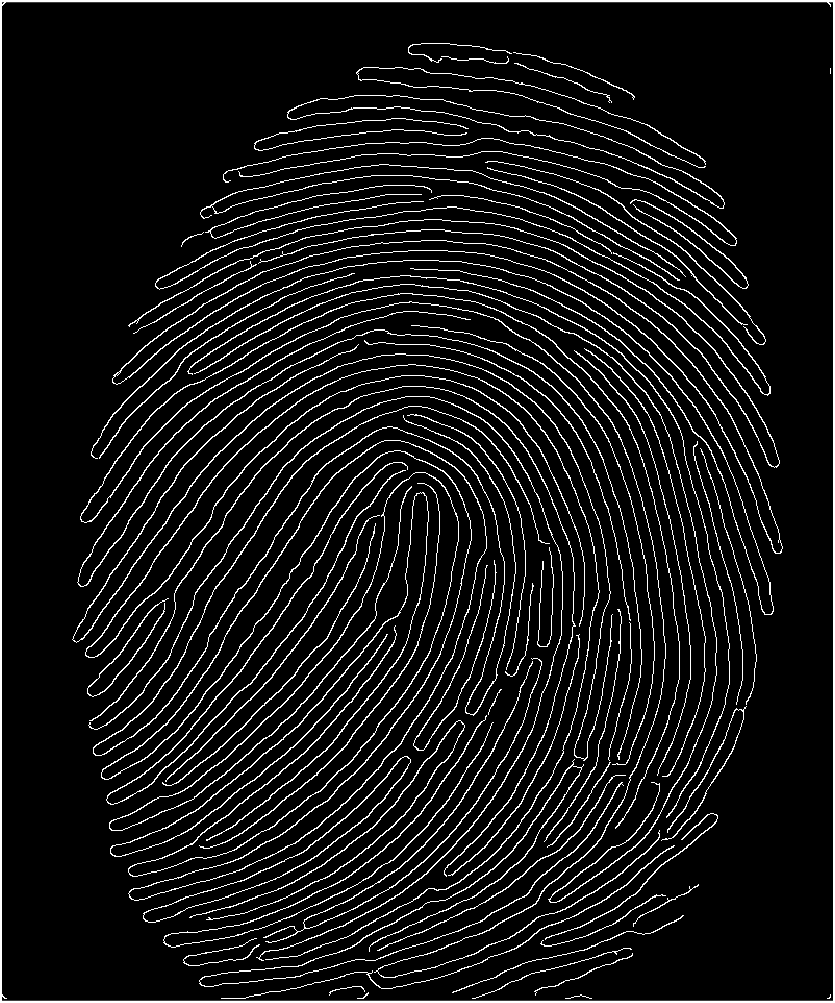
\includegraphics[height=0.4\textwidth]{../images/p1c/p1c}
	\caption{Edge tracking using Canny Edge Detector}
	\label{fig:p1c}
\end{figure}
\clearpage


\subsection*{Problem 2 (20 pts) }

Figure 1 shows an image of some texts titled with an unknown angle. For better readability, the titling angle must be found and used to correct the orientation of the image. Hough transform is a good choice for this application. ’tilted.png’ is one of the texts, your tasks are:
\begin{figure}[H]
	\centering 
	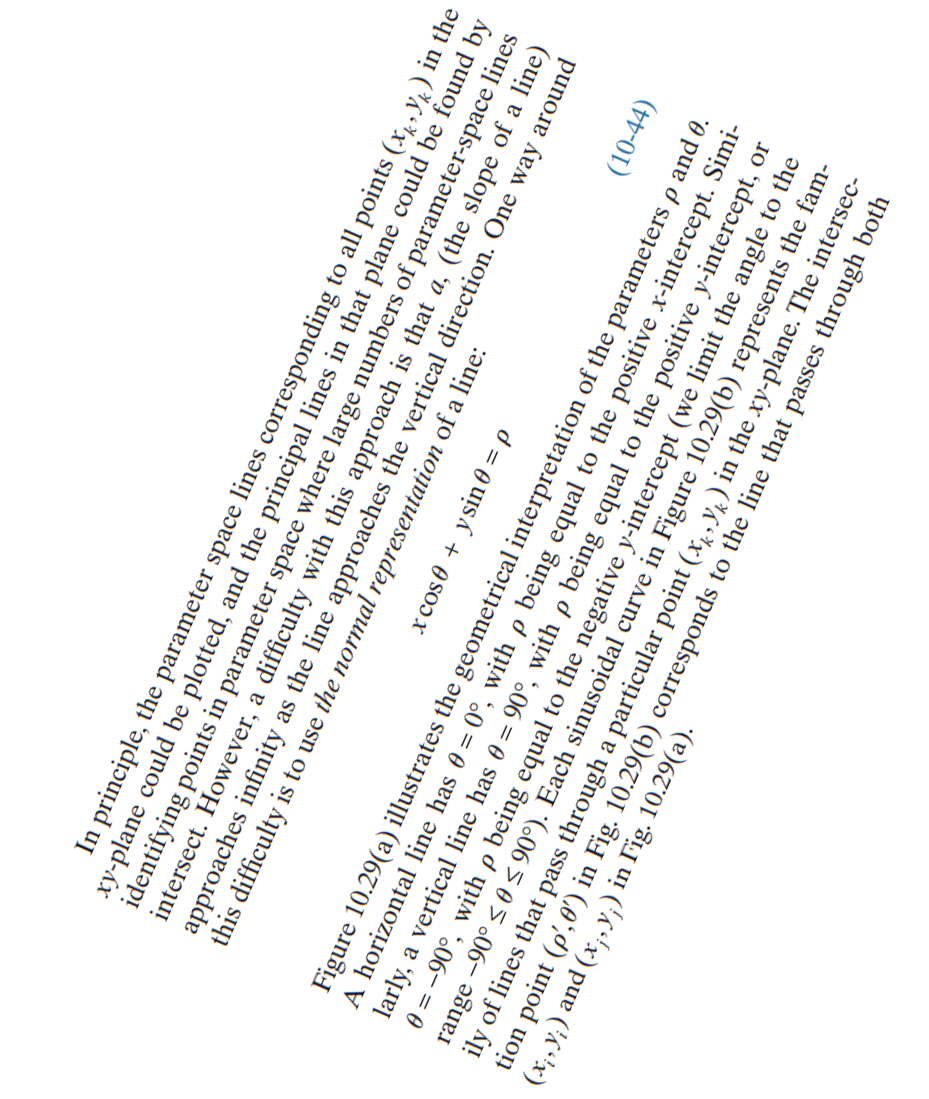
\includegraphics[width=0.5\textwidth]{tilted.PNG}
	\caption{tilted text}
	\label{Figure1}
\end{figure}
\begin{itemize}
\item[(a)] Implement Hough transform and perform it on ’tilted.png’, show its $\rho \theta$ -plane image. The input of Hough transform is a binary image, so you should do some thresholding before performing Hough transform. (15 pts)

\item[(b)] Using result obtained by Hough transform, correct the tilt angle, show the corrected image. (5 pts)

\end{itemize}
\textbf{Solution:}
\begin{itemize}
	\item [(a)] The $\rho \theta$ -plane image is shown in Figure~\ref{fig:p2a}. The binary thresholding is 0.7 (most words need to be set to 1).
				The $\Delta\rho$ is 2.5 and the  $\Delta\theta$ is 0.125. 
	\item [(b)] The corrected image is shown in Figure~\ref{fig:p2b}. Since the angle that perpendicular to the text line should contains largest values in accumulator,
				so I select the $\theta$ that has maximial value in accumulator.
\end{itemize}
\begin{figure}
	\centering
	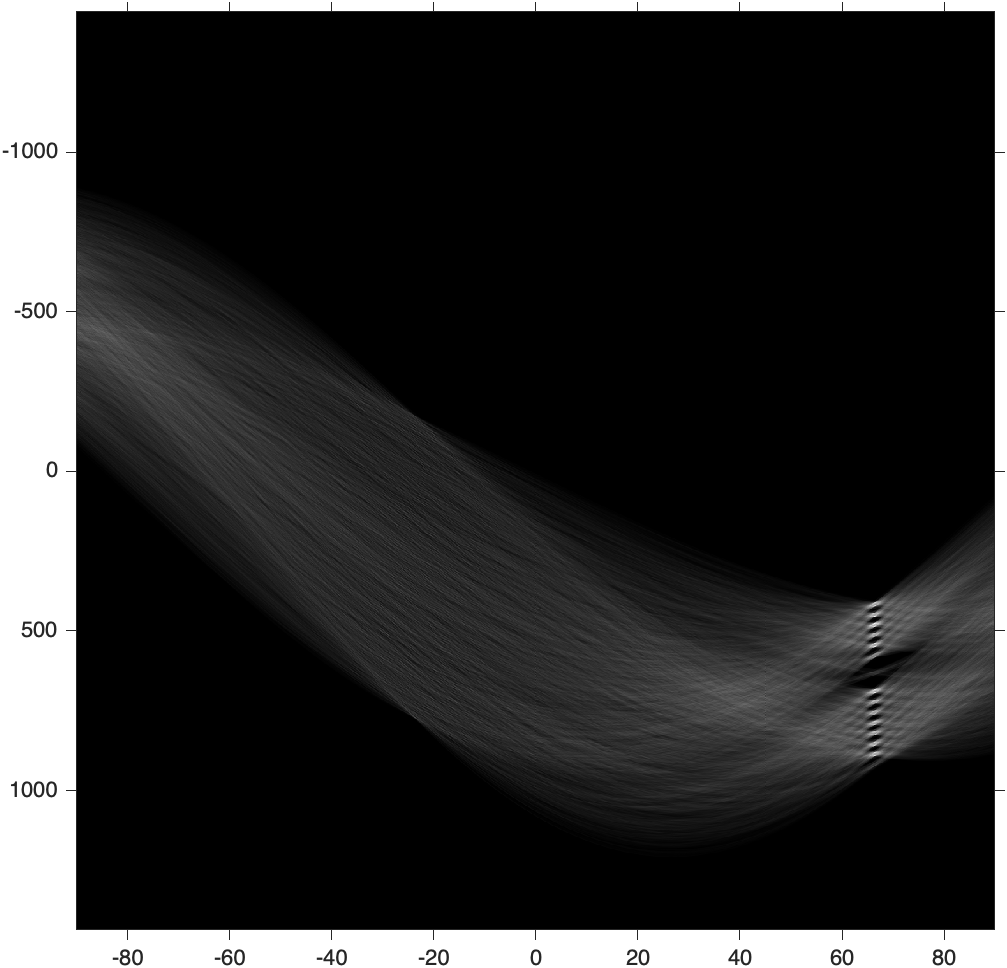
\includegraphics[width=0.5\textwidth]{../images/p2/p2a}
	\caption{Hough transform  of tilted tex}
	\label{fig:p2a}
	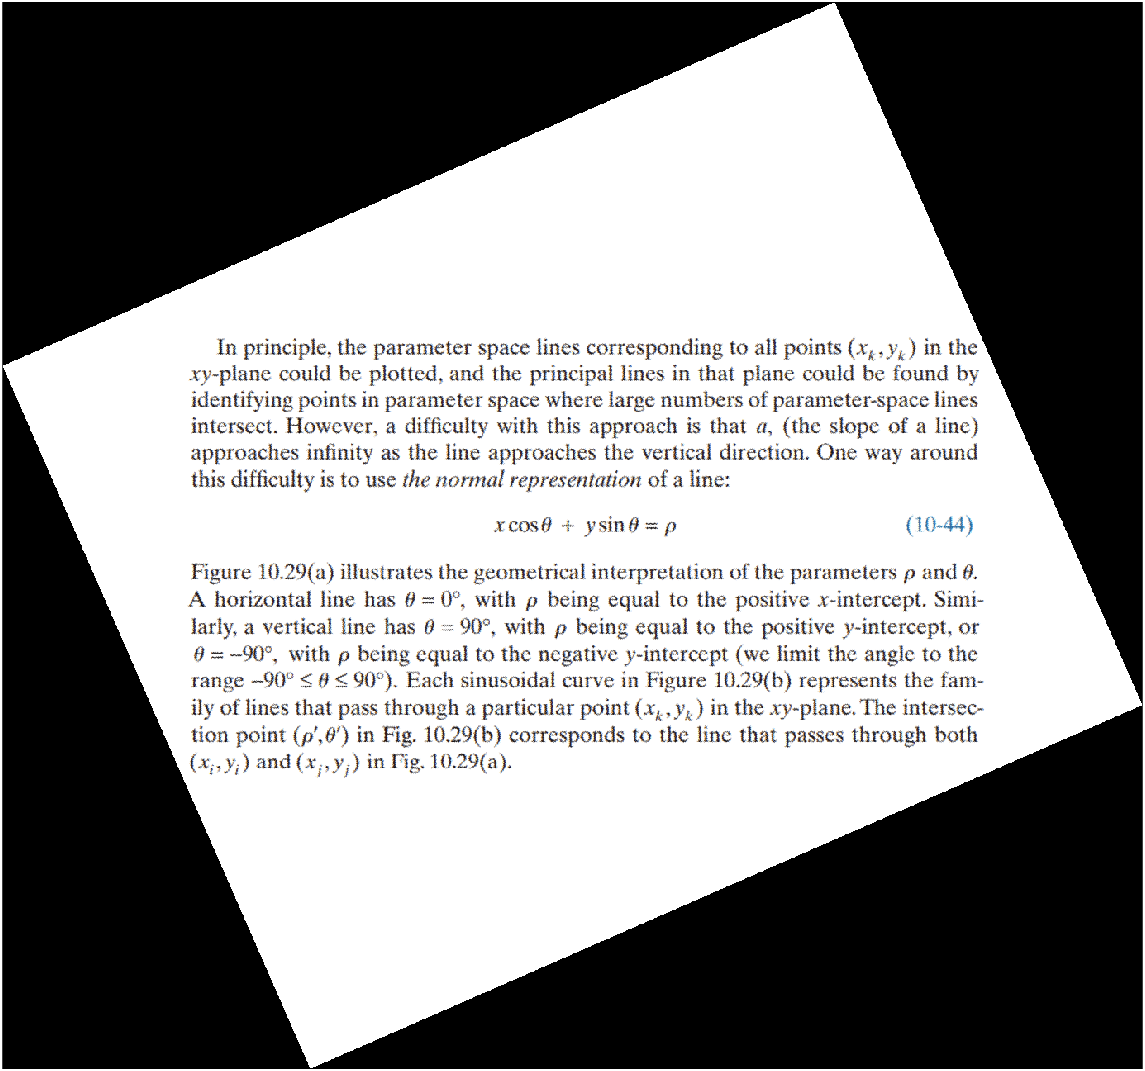
\includegraphics[width=0.5\textwidth]{../images/p2/p2b}
	\caption{Corrected image}
	\label{fig:p2b}
\end{figure}
\clearpage

\subsection*{Problem 3 (30 pts)}

Super pixel is a method that turns a pixel-level picture into district-level picture, which is an abstraction of basic information elements. A super pixel is a small area composed of a series of adjacent pixels with similar character-istics such as color, brightness, and texture. Most of these small areas retain effective information for further image segmentation, and generally do not destroy the boundary information of objects in the image.

In this problem, you need to turn ’sea house.jpg’ to super pixel style using SLIC algorithm with 100, 500 and 1000 cluster centers (In practice, number of cluster center can be slightly different from these values) and show the result images.

Reference, doi:10.1109/TPAMI.2012.120

\begin{figure}[H]
	\centering 
	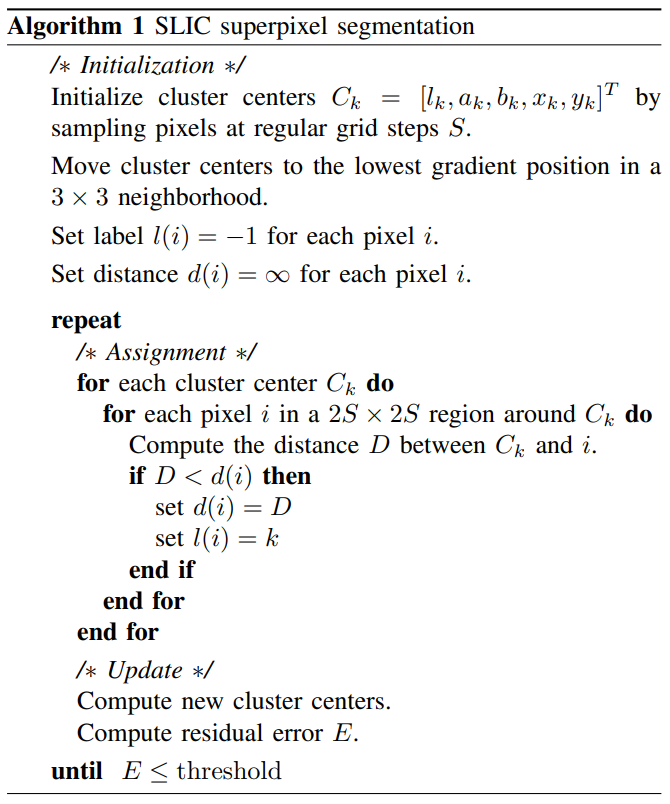
\includegraphics[width=0.5\textwidth]{SLIC.png}
	\caption{SLIC Algorithm}
	\label{Figure2}
\end{figure}

\begin{figure}[H]
	\centering 
	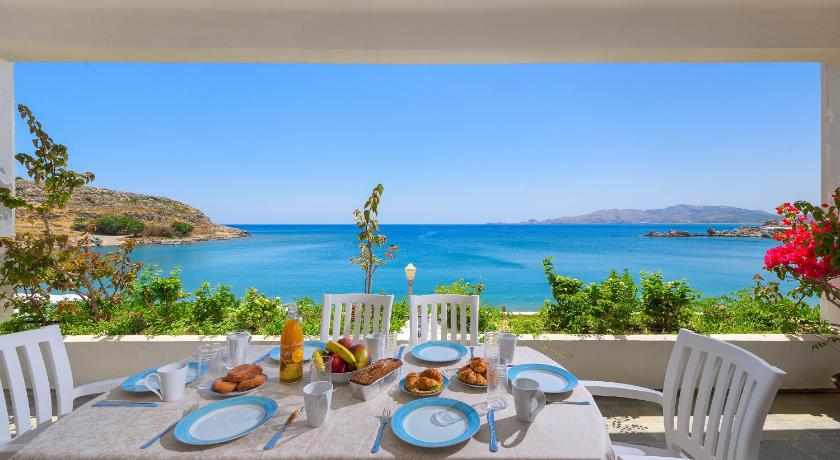
\includegraphics[width=0.5\textwidth]{sea_house.jpg}
	\caption{sea house.jpg}
	\label{Figure3}
\end{figure}
\textbf{Solution:}
The results with 100, 500 and 1000 cluster centers are shwon in Figure ~\ref{k_100}, Figure~\ref{k_500} and Figure~\ref{k_1000}.
\begin{figure}[hptb]
	\centering
	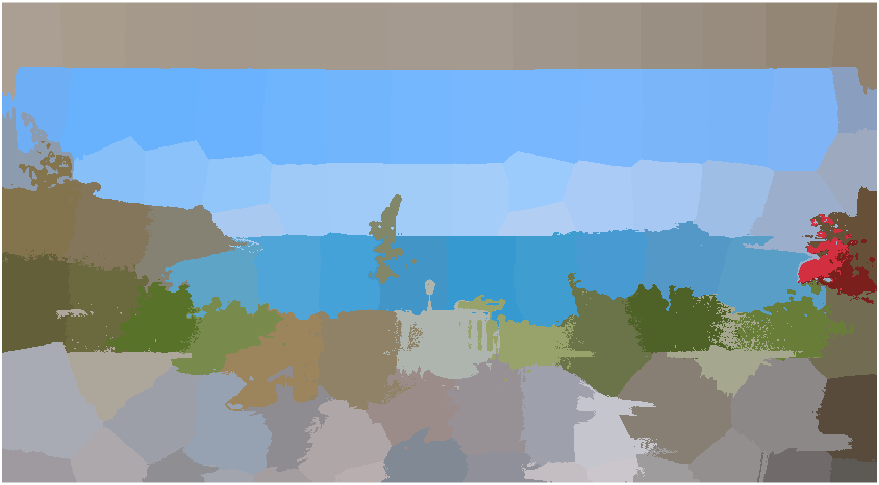
\includegraphics[width=0.5\textwidth]{../images/p3/k_100_t_0.5_m_40.png}
	\caption{cluster=100,threshold=0.5,m=40}
	\label{k_100}
	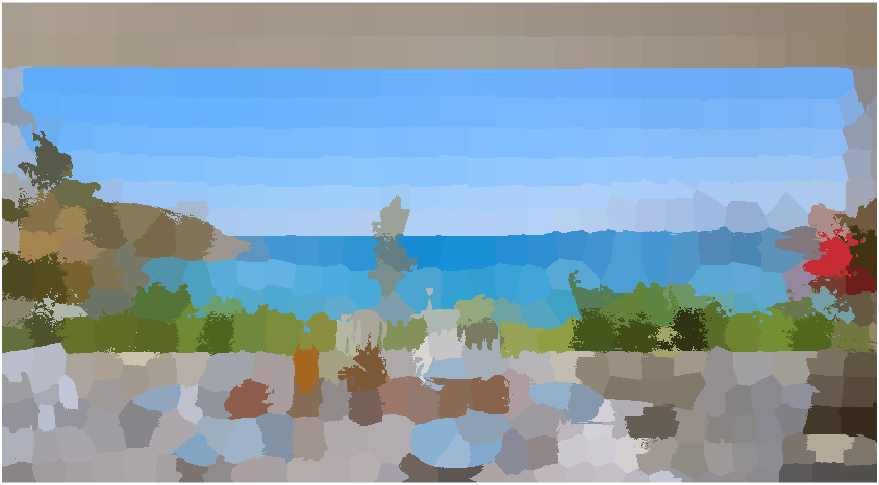
\includegraphics[width=0.5\textwidth]{../images/p3/k_500_t_0.5_m_40.png}
	\caption{cluster=500,threshold=0.5,m=40}
	\label{k_500}
	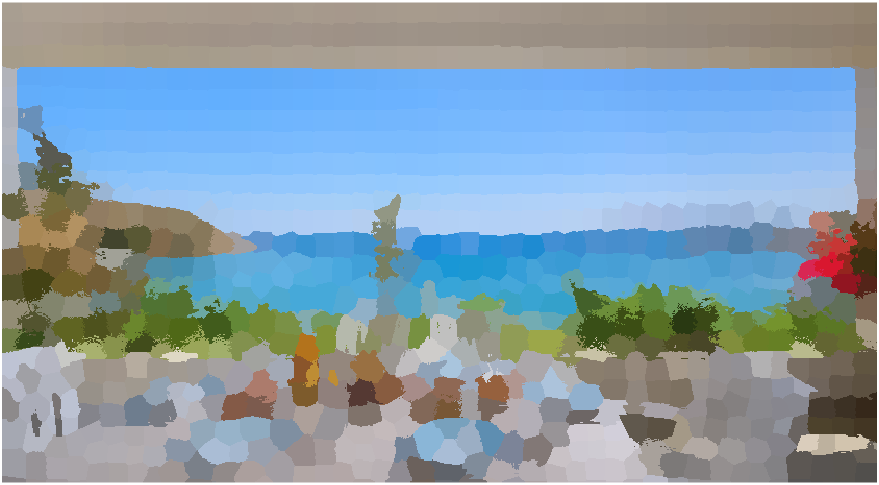
\includegraphics[width=0.5\textwidth]{../images/p3/k_1000_t_0.5_m_40.png}
	\caption{cluster=1000,threshold=0.5,m=40}
	\label{k_1000}
\end{figure}
\end{document}
